\subsection{Experiment 3: Reconstruction}

The AUDA analysis table is highly sparse due to substantial missing data across countries, regions, and years. For example, the United States Environmental Protection Agency (EPA) reports plastic waste generation data only at five-year intervals between 2000 and 2015. Therefore, in Experiment 3, we reconstruct the missing values in the \texttt{YearTRC (Japan)} and \texttt{YearTRC (US)} datasets.

The experiment compares simple interpolation baselines with statistical and machine-learning reconstruction models. Linear interpolation, moving average interpolation, and cubic spline interpolation provide reference methods for filling interior gaps. Ridge regression, Gaussian process regression (GPR), support vector regression (SVR), and Theil--Sen regression test whether fitted regression models can better capture the local trend in sparse country-level series.

Because both datasets have only 9 data points, each run uses only two held-out observations for testing. In this case, the denominator of \(R^2\) is very small, and modest absolute errors can produce a large negative \(R^2\). For this reason, the \(R^2\) metric is not very meaningful in this case, and we do not report it.

\begin{table}[!ht]
	\centering
	\caption{\centering Reconstruction performance for polymer PET consumption in Japan using the \texttt{YearPPC (Japan)} dataset, averaged over 16 runs.}
	\begin{tabular}{@{}lccccc@{}}
		\toprule
		\textbf{Experiment}         & \textbf{MAE}                   & \textbf{RMSE}         & $\mathbf{R^2}$ & \textbf{WAPE} & \textbf{MAPE} \\
		\midrule
		Linear Interpolation        & \(9.814 \times 10^4\)          & \(1.153 \times 10^5\)          & -130.623              & 2.65\%              & 2.64\%              \\
		Moving Average Interpolation & \(9.776 \times 10^4\)          & \(1.007 \times 10^5\)          & -99.532               & 2.64\%              & 2.64\%              \\
		Cubic Spline Interpolation  & \(6.101 \times 10^4\)          & \(7.454 \times 10^4\)          & -54.037               & 1.65\%              & 1.64\%              \\
		Ridge Regression            & \(9.569 \times 10^4\)          & \(9.708 \times 10^4\)          & -92.357               & 2.58\%              & 2.58\%              \\
		Gaussian Process Regression & \(1.059 \times 10^5\)          & \(1.180 \times 10^5\)          & -136.926              & 2.86\%              & 2.85\%              \\
		\textbf{Support Vector Regression} & \(\mathbf{2.938 \times 10^4}\) & \(\mathbf{4.094 \times 10^4}\) & \(\mathbf{-15.605}\) & \(\mathbf{0.79}\)\% & \(\mathbf{0.80}\)\% \\
		Theil-Sen Regression        & \(1.013 \times 10^5\)          & \(1.215 \times 10^5\)          & -145.342              & 2.73\%              & 2.73\%              \\
		\hline
	\end{tabular}
	\label{tab:reconstruction_japan_trc}
\end{table}

\begin{table}[!ht]
	\centering
	\caption{\centering Reconstruction performance for total resin consumption in the United States using the \texttt{YearTRC (US)} dataset, averaged over 16 runs.}
	\begin{tabular}{@{}lccccc@{}}
		\toprule
		\textbf{Experiment}                & \textbf{MAE}                   & \textbf{RMSE}                  & $\mathbf{R^2}$       & \textbf{WAPE}       & \textbf{MAPE}       \\
		\midrule
		Linear Interpolation               & \(1.141 \times 10^5\)          & \(1.553 \times 10^5\)          & 0.923                & 0.79\%              & 0.76\%              \\
		Moving Average Interpolation       & \(1.313 \times 10^5\)          & \(1.471 \times 10^5\)          & 0.931                & 0.91\%              & 0.92\%              \\
		Cubic Spline Interpolation         & \(2.469 \times 10^5\)          & \(2.630 \times 10^5\)          & 0.778                & 1.70\%              & 1.68\%              \\
		Ridge Regression                   & \(1.872 \times 10^5\)          & \(1.883 \times 10^5\)          & 0.886                & 1.29\%              & 1.29\%              \\
		\textbf{Gaussian Process Regression} & \(\mathbf{7.875 \times 10^4}\) & \(\mathbf{8.323 \times 10^4}\) & \(\mathbf{0.978}\)  & \(\mathbf{0.54}\)\% & \(\mathbf{0.54}\)\% \\
		Support Vector Regression          & \(2.655 \times 10^5\)          & \(2.670 \times 10^5\)          & 0.771                & 1.83\%              & 1.83\%              \\
		Theil-Sen Regression               & \(1.576 \times 10^5\)          & \(1.592 \times 10^5\)          & 0.919                & 1.09\%              & 1.10\%              \\
		\hline
	\end{tabular}
	\label{tab:reconstruction_united_states_trc}
\end{table}

\begin{figure}[H]
	\centering

	\subfloat[\texttt{YearTRC (Japan)} with ridge regression.]{
		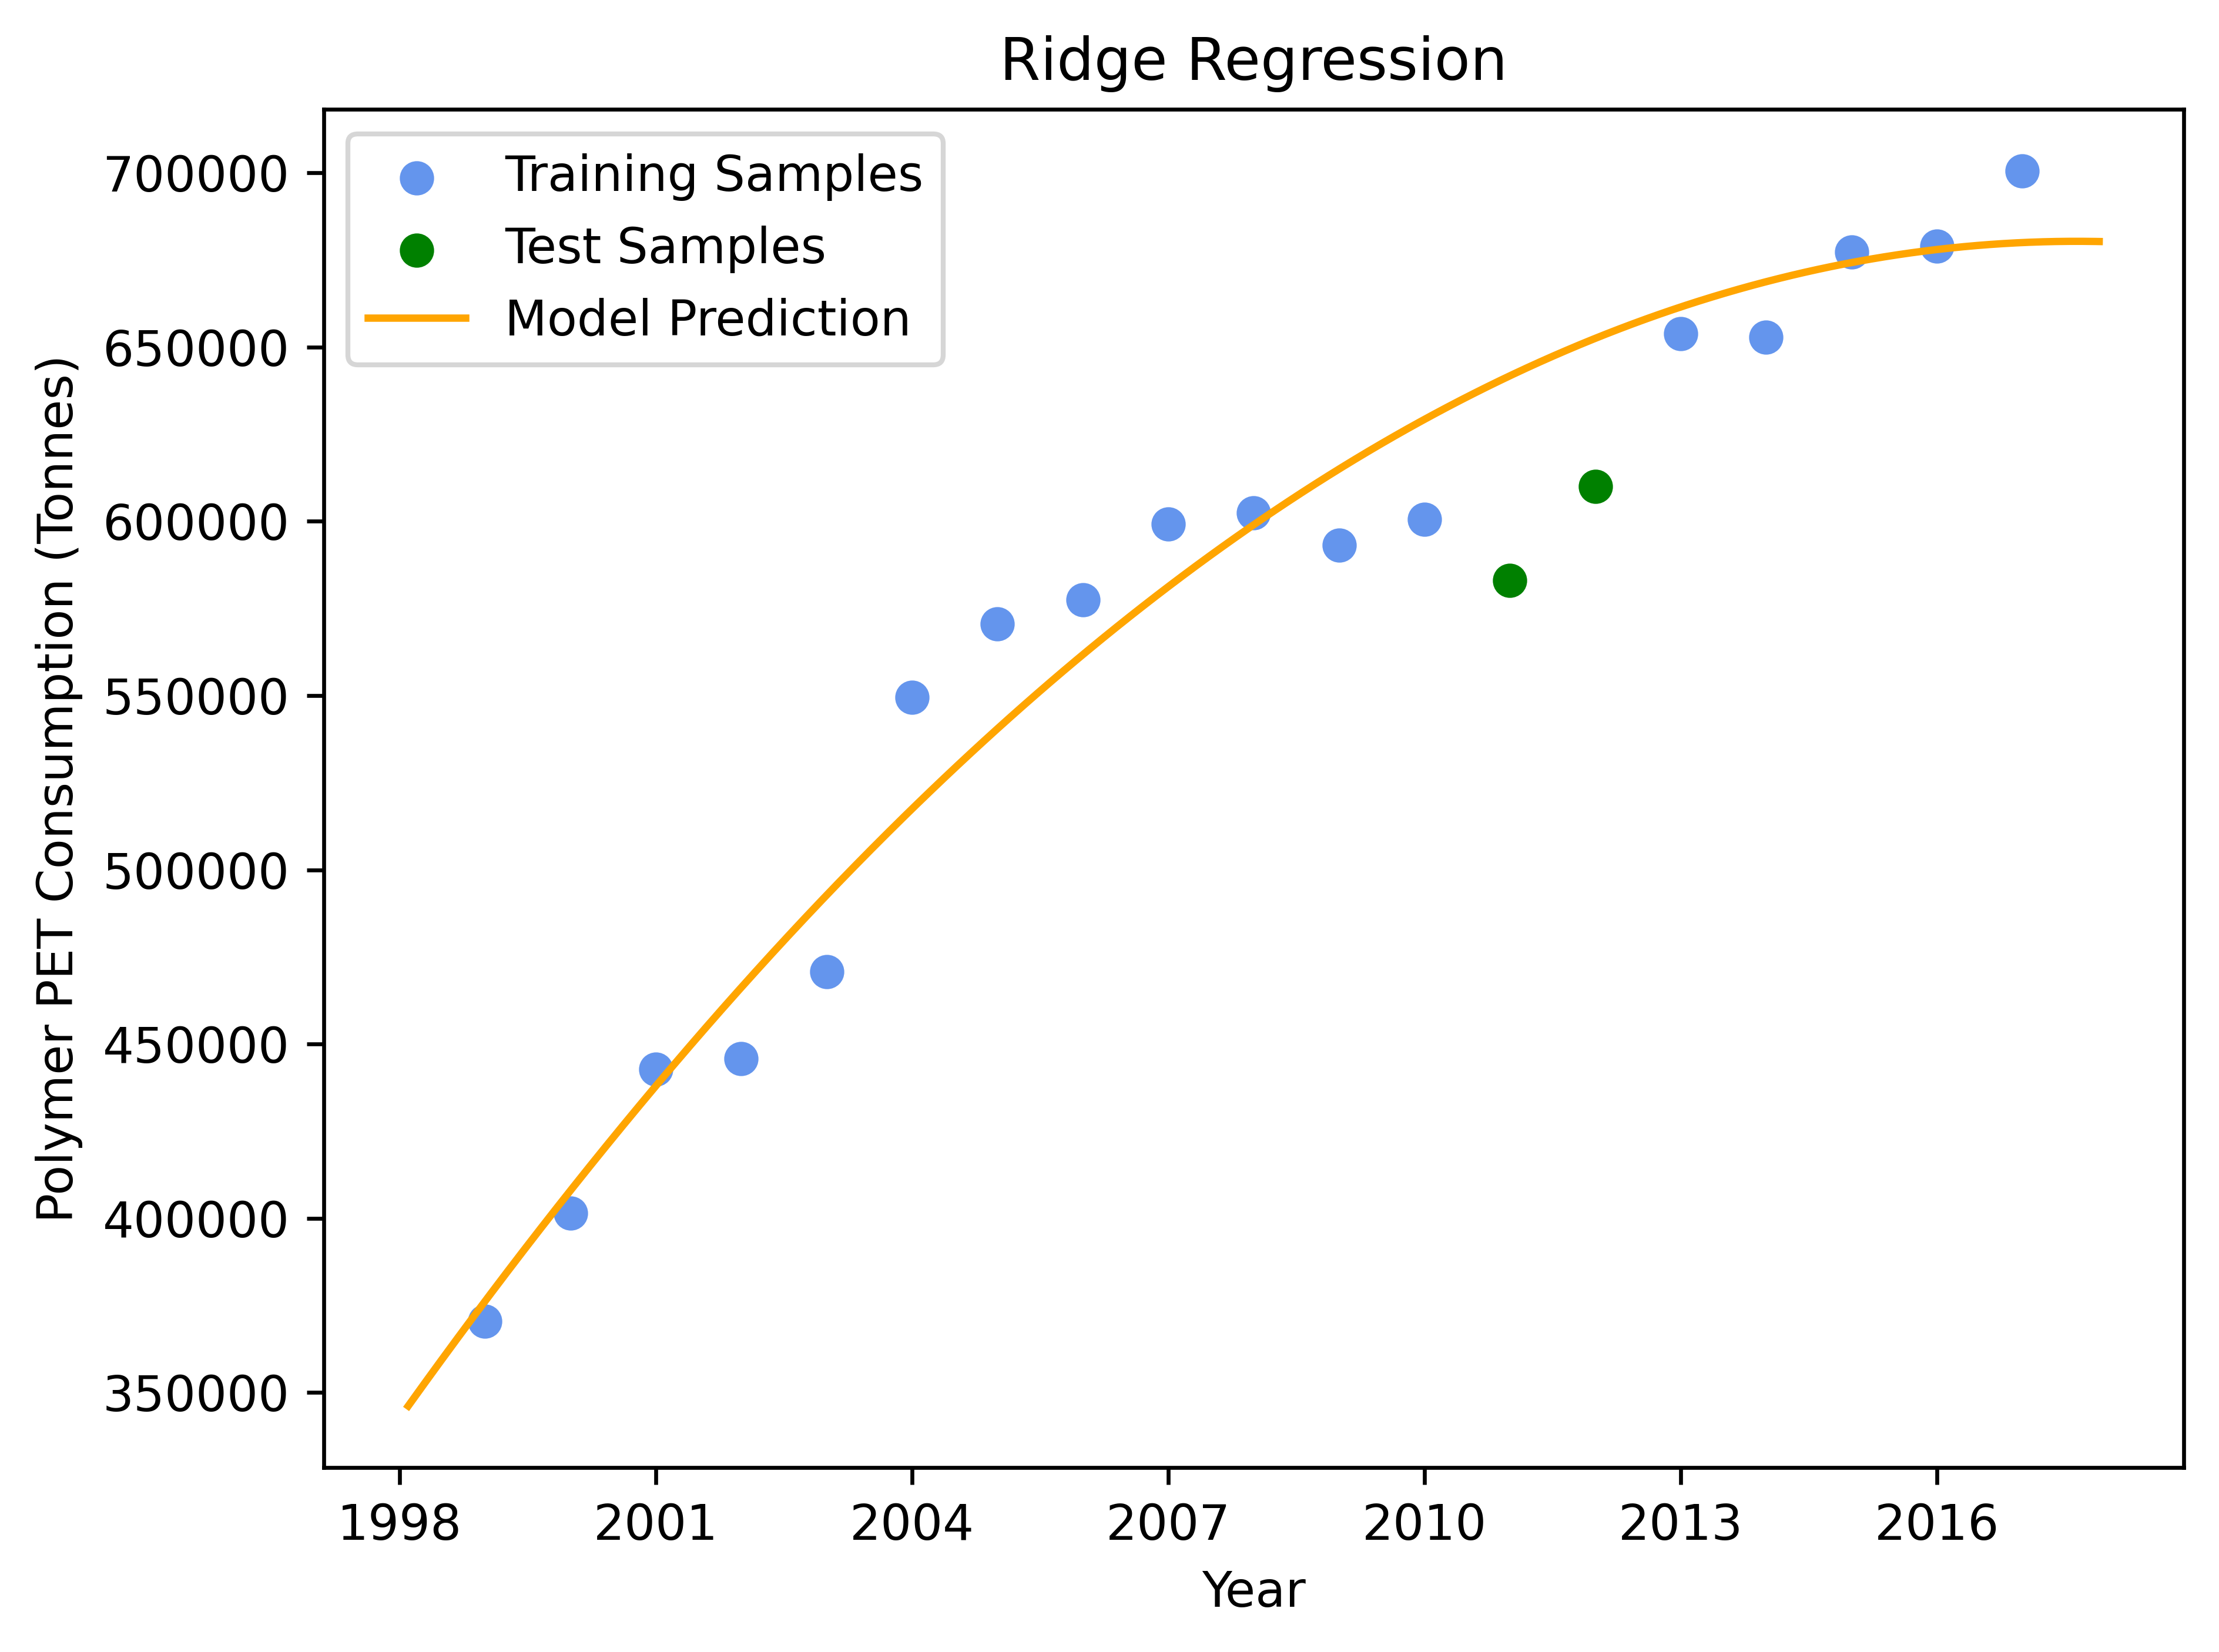
\includegraphics[width=0.45\textwidth]{figures/japan_trc_reconstruction_ridge_regression.png}
	}
	\subfloat[\texttt{YearTRC (Japan)} with SVR.]{
		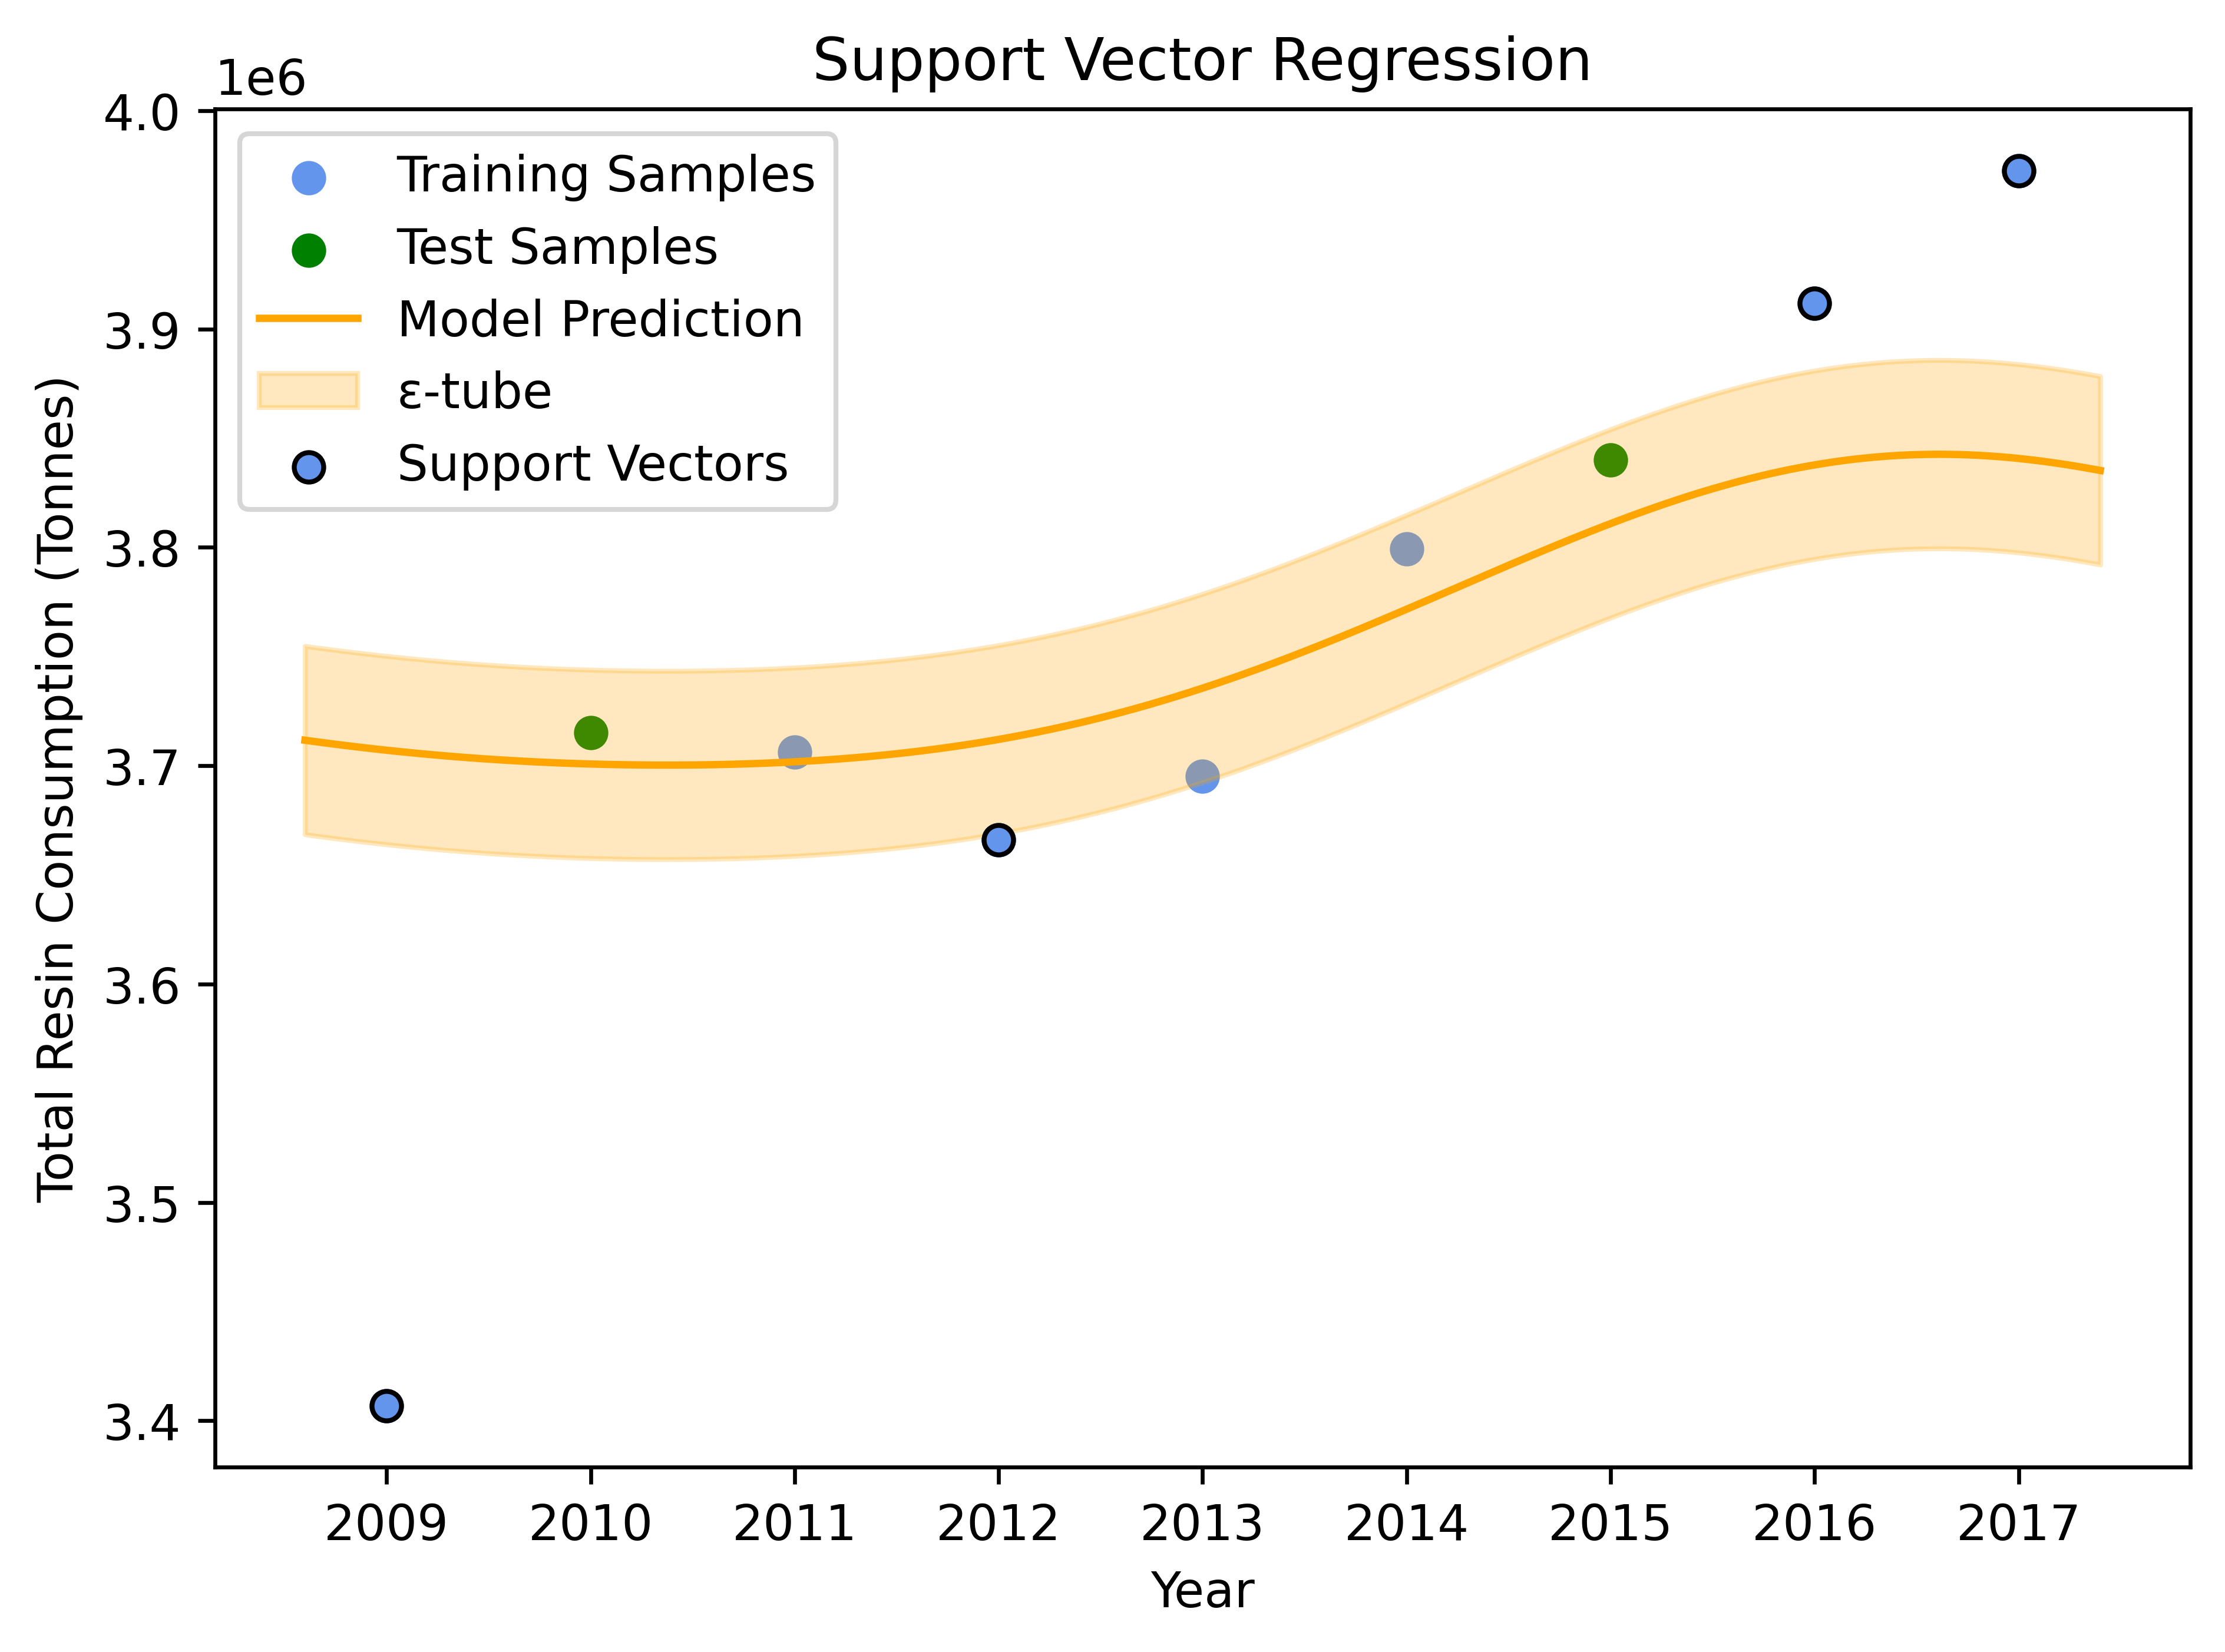
\includegraphics[width=0.45\textwidth]{figures/japan_trc_reconstruction_svr.png}
	}

	\vspace{0.5cm}

	\subfloat[\texttt{YearTRC (United States)} with GPR.]{
		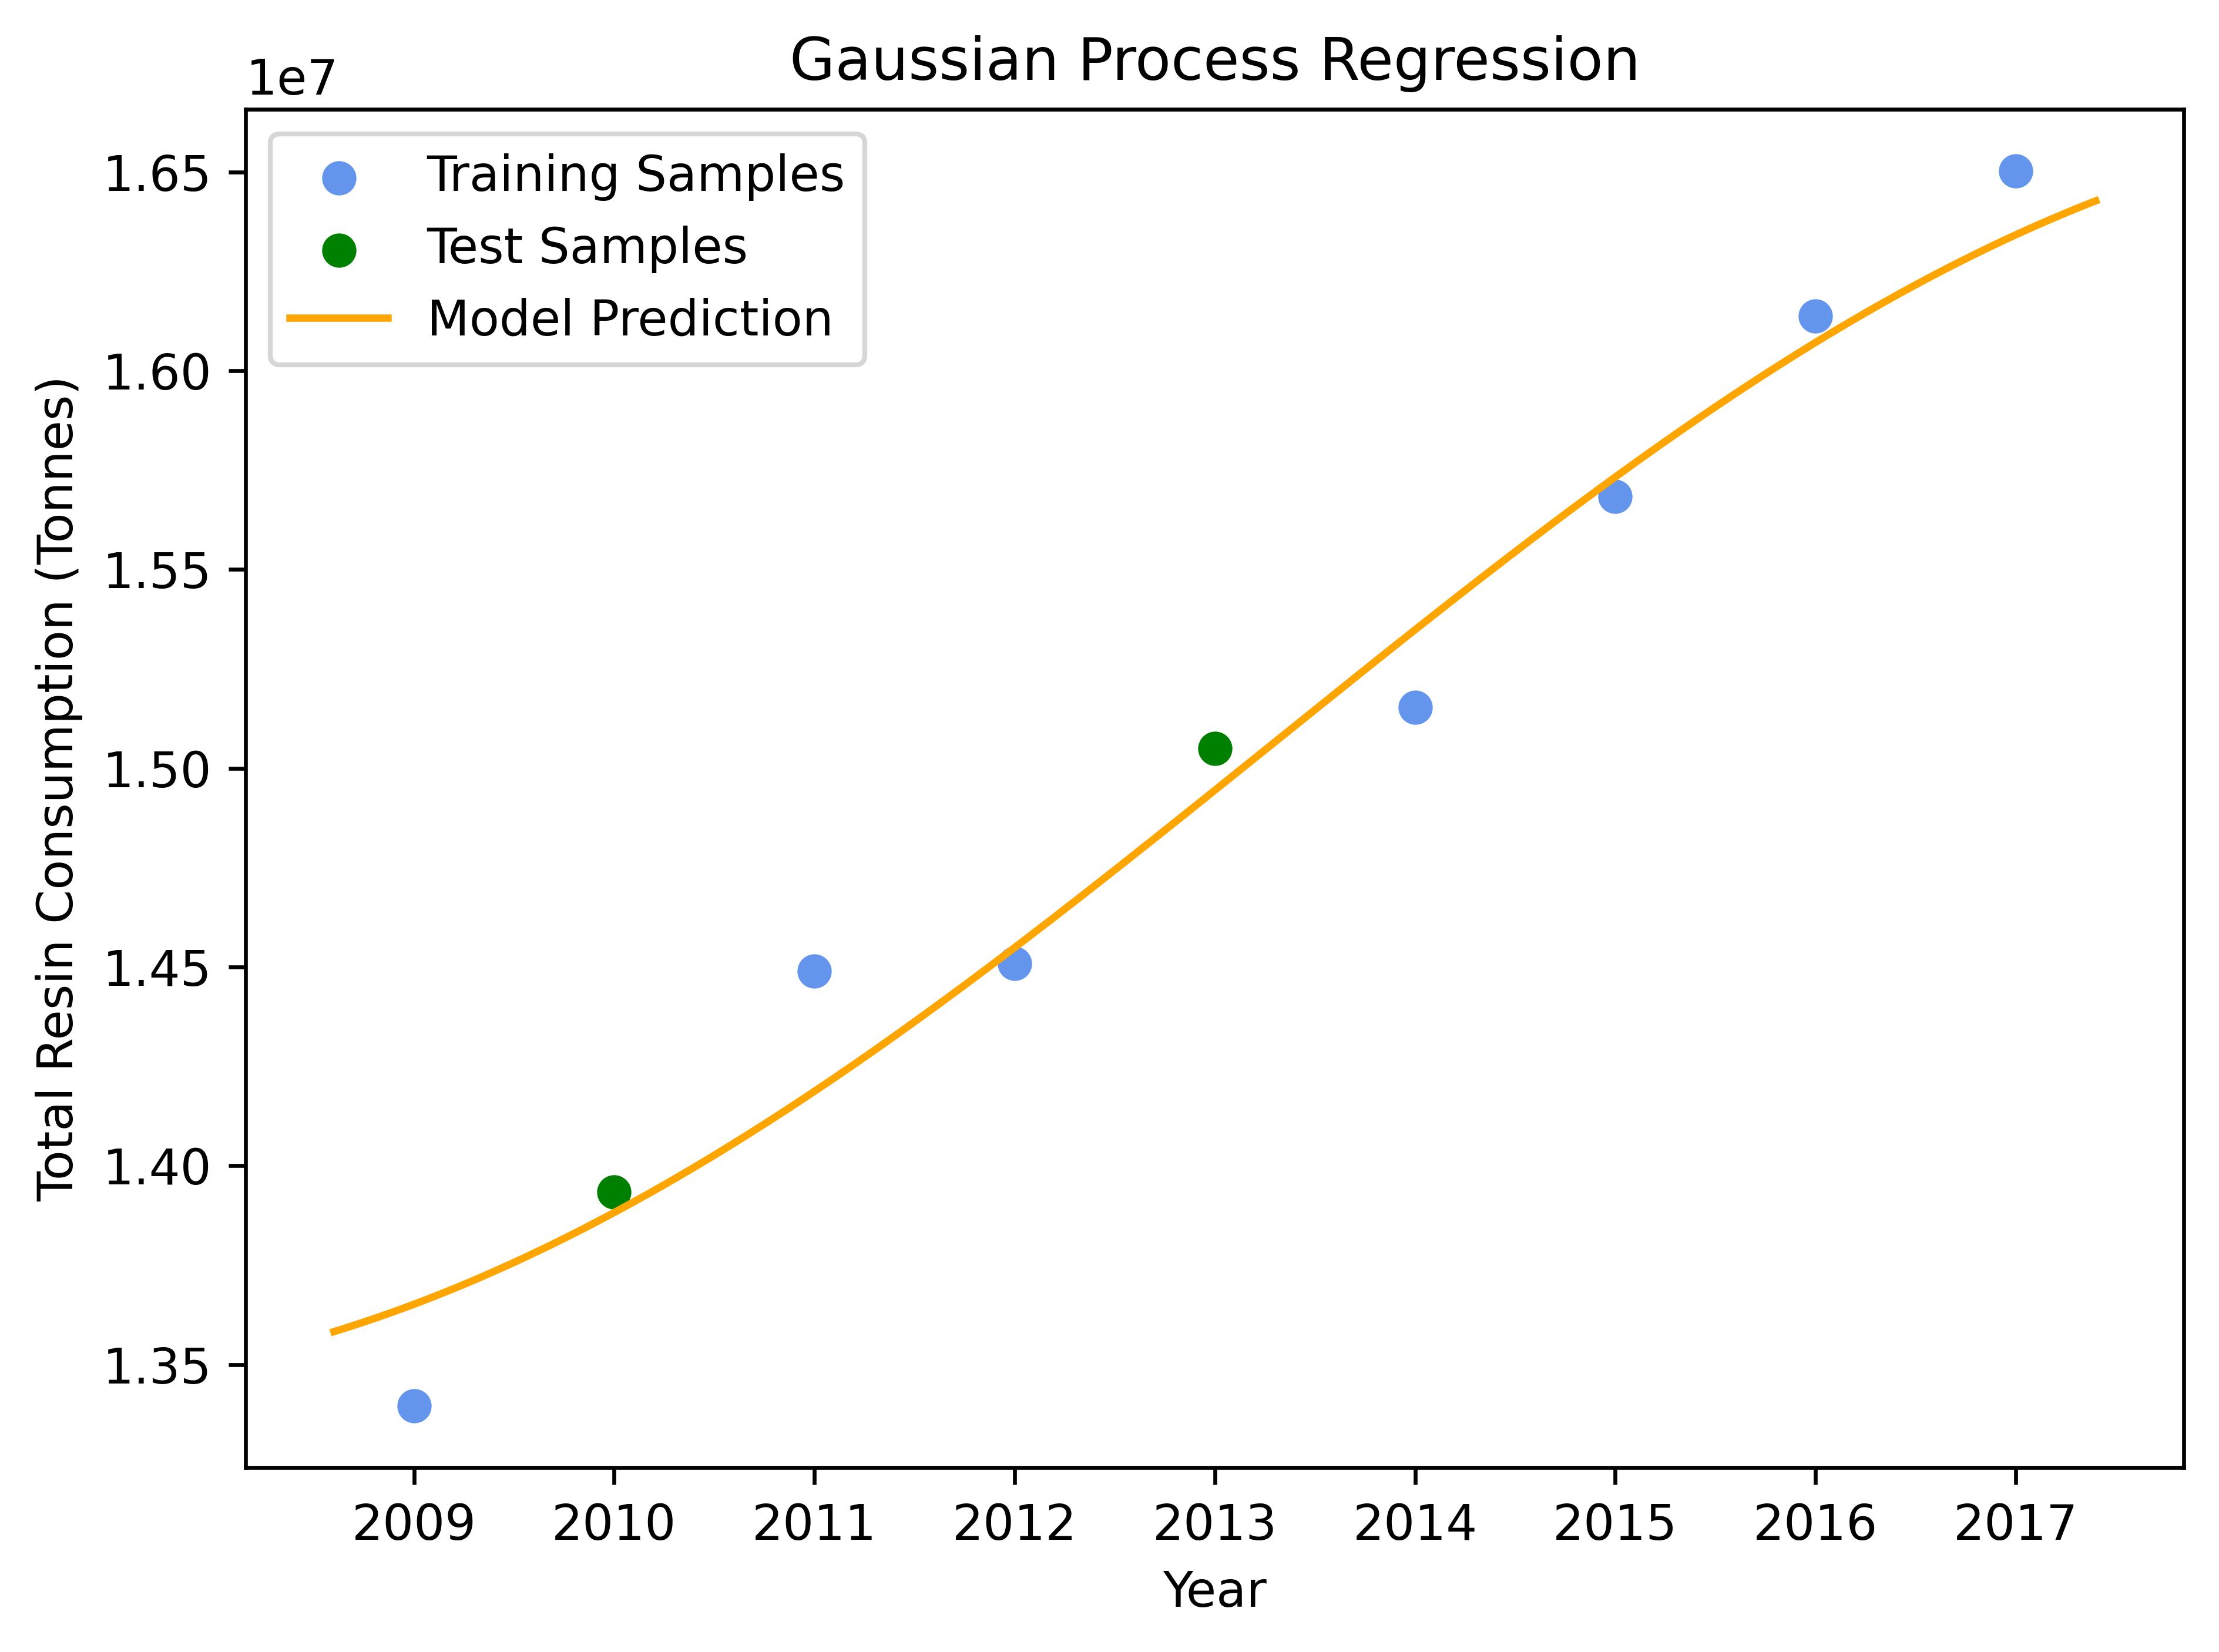
\includegraphics[width=0.45\textwidth]{figures/united_states_ppc_reconstruction_gpr.png}
	}
	\hfill
	\subfloat[\texttt{YearTRC (United States)} with SVR.]{
		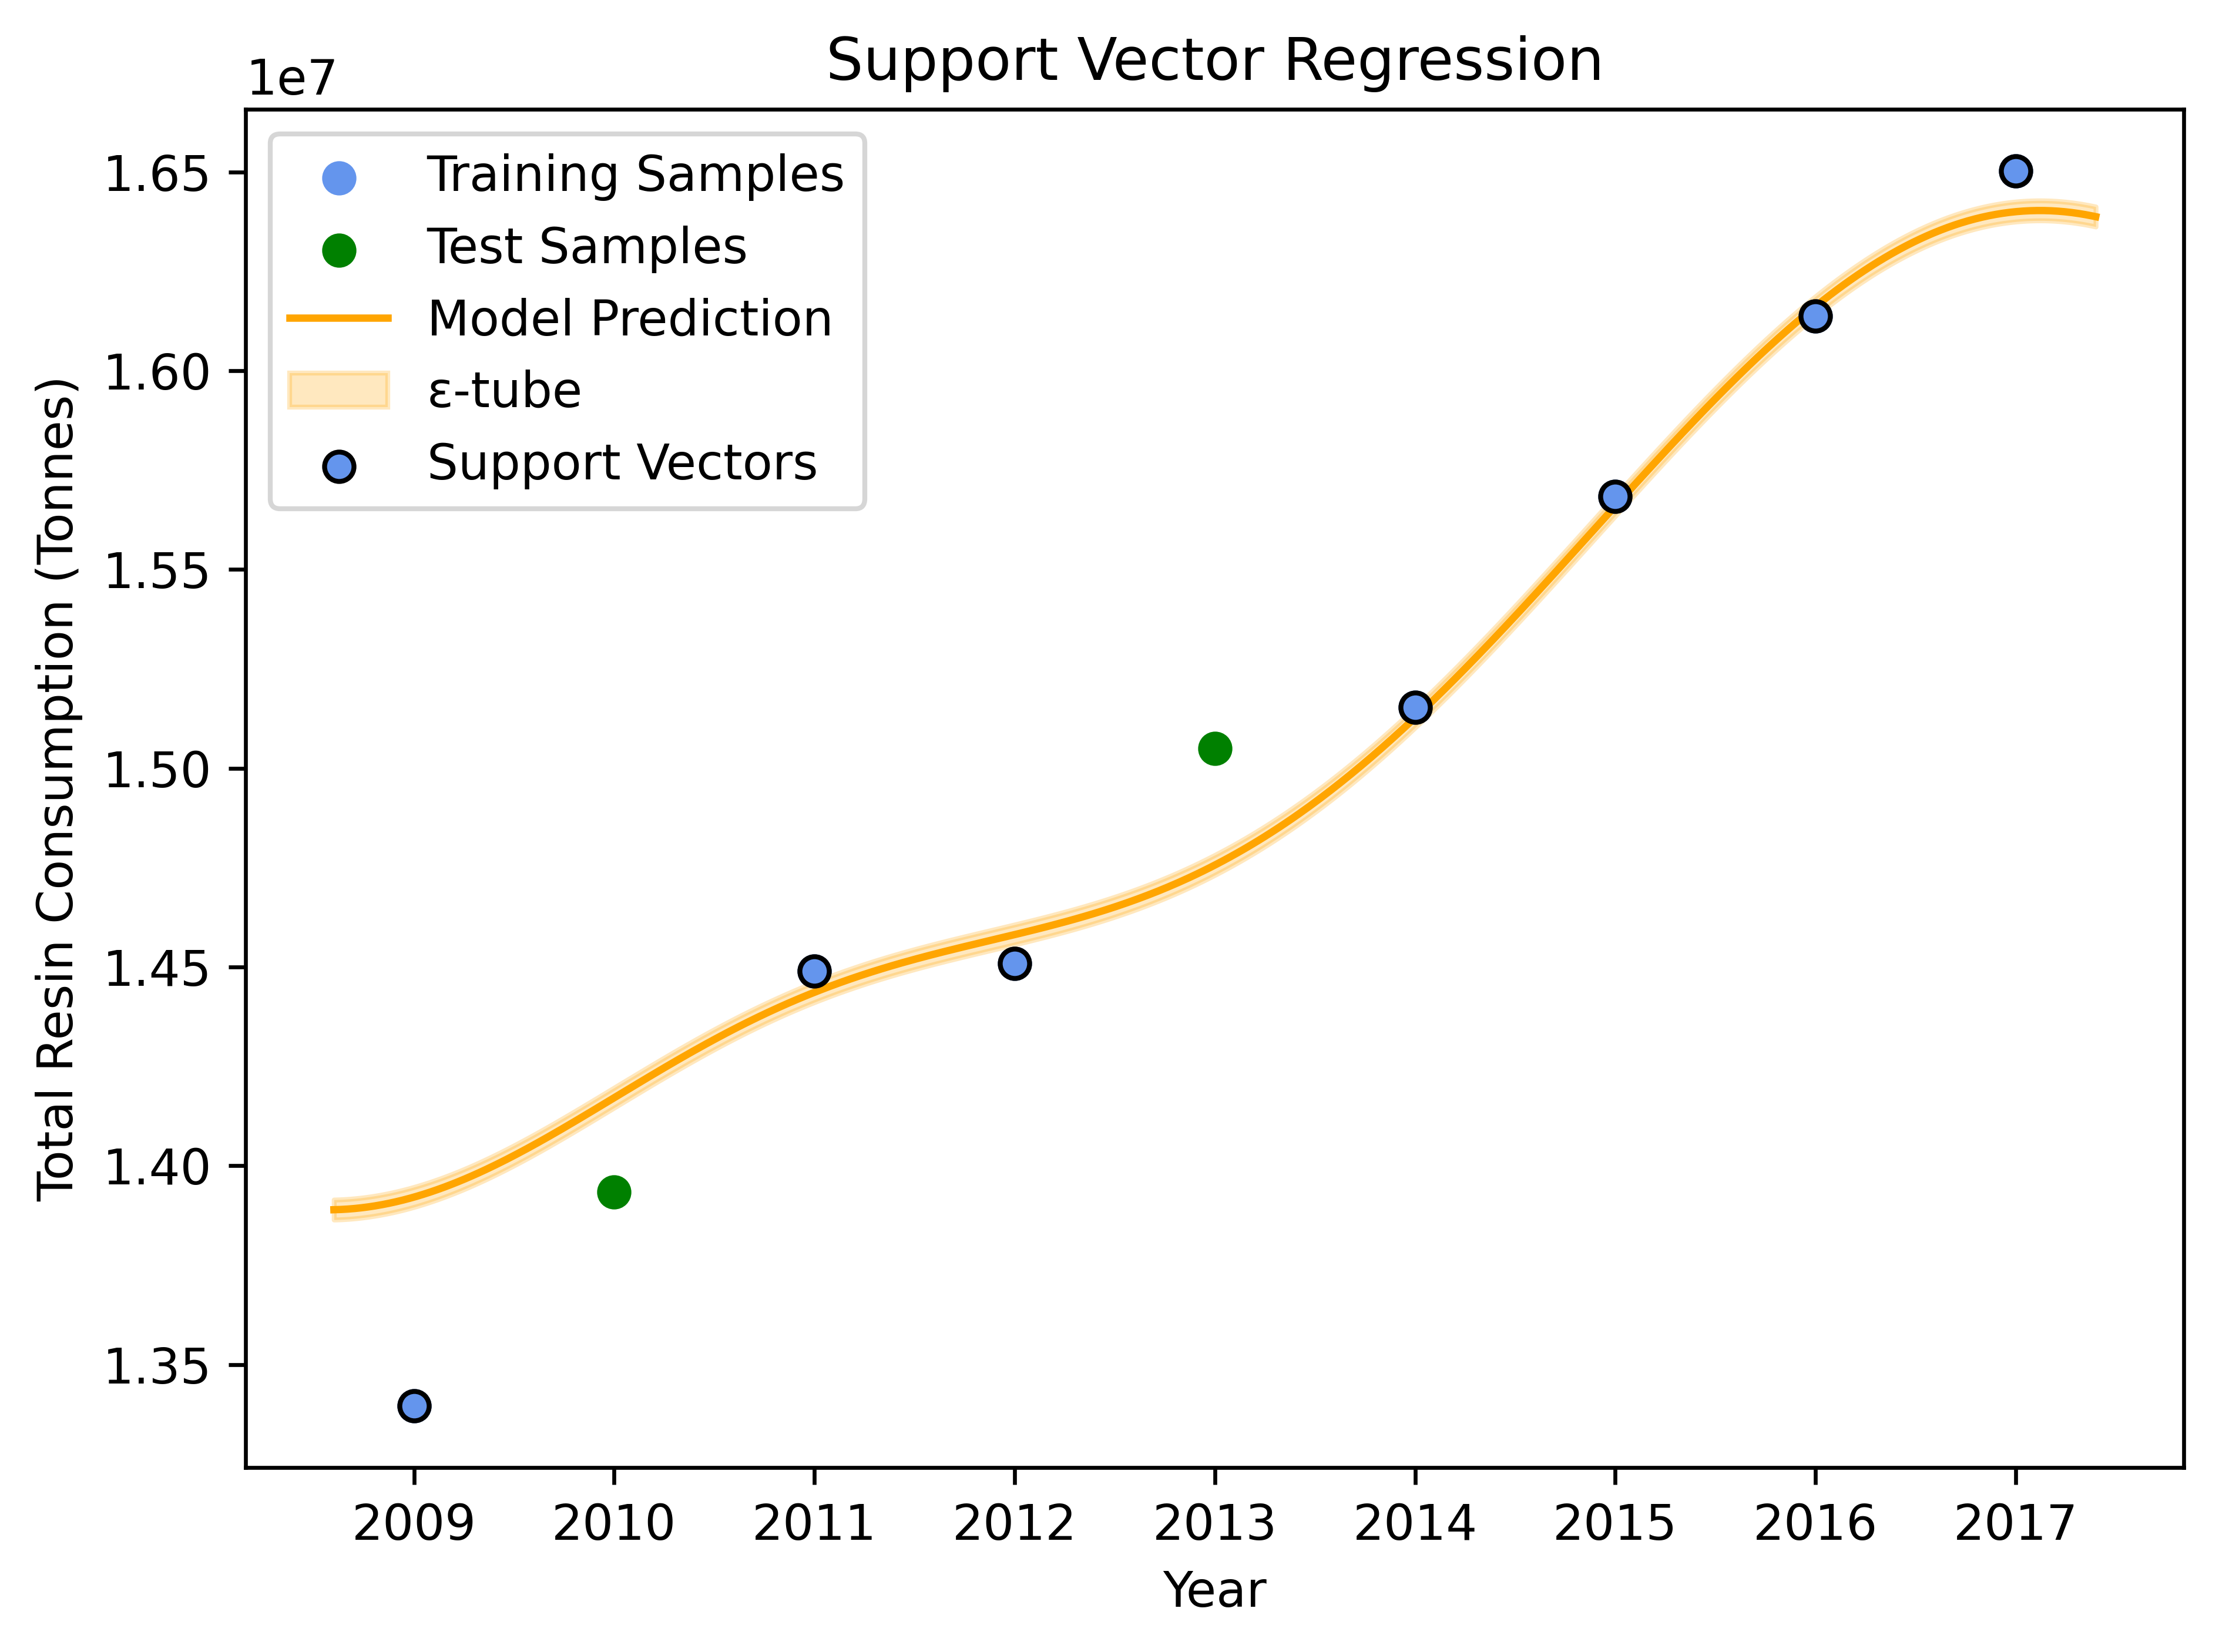
\includegraphics[width=0.45\textwidth]{figures/united_states_ppc_reconstruction_svr.png}
	}

	\caption{Reconstruction plots for the \texttt{YearTRC} dataset: ridge regression and SVR for Japan, and GPR and SVR for the United States.}

	\label{fig:reconstruction_plots}
\end{figure}


% A
Table~\ref{tab:reconstruction_japan_trc} shows that SVR performs best on the \texttt{YearTRC (Japan)} reconstruction task, achieving the lowest MAE, RMSE, and WAPE among the evaluated methods. Its WAPE is 1.36\%, compared with 1.48\% for cubic spline interpolation and 1.59\% for linear interpolation. This suggests that the Japan series benefits from a flexible nonlinear model.

Table~\ref{tab:reconstruction_united_states_trc} shows a slightly different pattern for the \texttt{YearTRC (US)} task. SVR gives the best overall result, with a WAPE of 1.08\%, while Theil--Sen regression and linear interpolation are also competitive at 1.17\% and 1.19\%, respectively. These results indicate that the United States series can be reconstructed accurately by both flexible machine learning models and smoother trend-based methods, and that the best model can vary across countries even when the target variable and reconstruction setup are similar.

Figure~\ref{fig:reconstruction_plots} shows representative fitted trajectories from the reconstruction experiments. The \texttt{YearTRC (Japan)} series exhibits a more nonlinear trend than the \texttt{YearTRC (US)} series, which may explain why SVR performs better for Japan, while Theil--Sen regression and linear interpolation perform better for the United States. However, because both series contain few samples and show local fluctuations, visual inspection alone is not enough to draw strong conclusions about the relative performance of the models.
